\documentclass[UTF8,a4paper,8pt]{ctexart} 

 \usepackage{graphicx}   %学习插入图
 \usepackage{verbatim}   %学习注释多行
 \usepackage{booktabs}   %表格
 \usepackage{geometry}   %图片
 \usepackage{amsmath} 
 \usepackage{amssymb}
 \usepackage{listings}   %代码
 \usepackage{xcolor}     %颜色
 \usepackage{enumitem}   %列表格式
 \usepackage{algorithm}  %format of the algorithm
 \usepackage{algorithmic}%format of the algorithm
 \usepackage{multirow}   %multirow for format of table
 \CTEXsetup[format+={\flushleft}]{section}
 
 
 \renewcommand{\algorithmicrequire}{\textbf{Input:}}   %Use Input in the format of Algorithm
 \renewcommand{\algorithmicensure}{\textbf{Output:}}   %UseOutput in the format of Algorithm
\geometry{left=1.6cm,right=1.8cm,top=2cm,bottom=1.7cm} %设置文章宽度

\pagestyle{plain} 		  %设置页面布局
\author{郑华}
\title{计算机动画}
 %代码效果定义
 
 \definecolor{codegreen}{rgb}{0,0.6,0}
 \definecolor{codegray}{rgb}{0.5,0.5,0.5}
 \definecolor{codepurple}{rgb}{0.58,0,0.82}
 \definecolor{backcolour}{rgb}{0.95,0.95,0.92}
 
 \lstdefinestyle{mystyle}{
 	language = {c++},%lua 语言指定方法
 	backgroundcolor=\color{backcolour},   
 	commentstyle=\color{codegreen},
 	keywordstyle=\color{magenta},
 	numberstyle=\tiny\color{codegray},
 	stringstyle=\color{codepurple},
 	basicstyle=\footnotesize,
 	breakatwhitespace=false,         
 	breaklines=true,                 
 	captionpos=b,                    
 	keepspaces=true,                 
 	%numbers=left,                    
 	%numbersep=5pt,                  
 	showspaces=false,                
 	showstringspaces=false,
 	showtabs=false,                  
 	tabsize=2
 }
\lstset{style=mystyle, escapeinside=``}

\begin{document}          %正文排版开始
 	\maketitle

\newpage
\section{面}  
   \paragraph{参数}
	   \begin{itemize}
		   	\item B样条曲线
		   	\item Nurbs 曲线
		   	\item ODE
		   	\item PDE
	   \end{itemize} 
	 
	 \paragraph{转换}
		 从二维到三维的转化,参数u,v 对应于2维的u
		 \begin{itemize}
		 	\item 可微
		 	\item 全部,高阶多项式
		 	\item 分段,低度多项式,连续性和可微性的
		 \end{itemize} 
		 
	 \paragraph{Bezier 曲面}
	 \paragraph{NURBs  曲面}
	 \paragraph{Subdivision 细分曲面-线}Subdivide each face of the polyhedron, to make a smooth surface
		 \subparagraph{Interpolating Schemes}Limit Surfaces/Curve \textbf{will pass through} original set of data points.
		 \subparagraph{Approximating Schemes}Limit Surface \textbf{will not necessarily pass} through the original set of data points
		 
		 \subparagraph{切角细分曲线 Corner Cutting Subdivision Curves}
		 
		 \begin{algorithm}[htb]
		 	\caption{切角 细分 曲线}
			\label{alg:CornerCut}
			\begin{algorithmic}[1]
				\REQUIRE ~~\\ 
				多点曲线 \\
				各点的坐标
				\ENSURE ~~\\
					细分后的曲线,实质是更多点组合起来的折线
										
				 \STATE 找到相邻的两个边
				 \STATE 取其共同顶点
				 \STATE 连接与这两条边(近)的1/3,即截取 
				 \STATE 迭代所有边
				 \STATE 直到满足要求
			\end{algorithmic}
		 \end{algorithm}
			 
		\begin{algorithm}[htb]
			\caption{外伸1/8 估计细分 曲线}
			\label{alg:Approximating Extends}
			\begin{algorithmic}[1]
				\REQUIRE ~~\\ 
				多点曲线 \\
				各点的坐标
				\ENSURE ~~\\
				细分后的曲线,实质是更多点组合起来的折线
				
				\STATE 随机确定一个边
				\STATE 找其连接的两个边的终点
				\STATE 取其两个的中点(两终点), 取其(原边)中点,求其距离d
				\STATE 并沿着该直线的方向外伸d/8 
				\STATE 迭代直到满足要求
			\end{algorithmic}
		\end{algorithm}
		
		\paragraph{细分曲面}细分曲面是对给定的多边形(控制多边形,控制网)进行不断的细分操作而产生的
			\begin{itemize}
				\item 收敛,极限曲面
				\item 平滑
				\item 在每次迭代中,细分操作细化了控制网,增加了大致4倍顶点的数量
				\item 每个细分方法都存在则 1个生成细分控制网络的拓扑结构的方法和1个确定新顶点位置的规则
			\end{itemize}
			\subparagraph{三角细分}
				将每个边细分为1,2,3,4,5....


\newpage				
\section{碰撞检测}
		\subsection{核心}
			\begin{itemize}
				\item 碰撞检测实质是一个几何交集检测问题
				\item 静态或动态-假设有两个移动对象定义了在最初和最终的状态,确定他们是否在两个状态之间的某一点相交
				\item Detection should be fast, from finding the candidate objects to one-one intersection test. O(n2)
				\item 从碰撞反弹 Response from the collision
			\end{itemize}
		
		\subsection{碰撞检测-静态}
			\paragraph{One-One}
				\begin{itemize}
					\item 简单形状检测
					\item 复杂形状检测
				\end{itemize}
				\subparagraph{简单形状测试}:
					\begin{figure}[h]
						\centering
						\caption{One-One Simple shape Testing}
						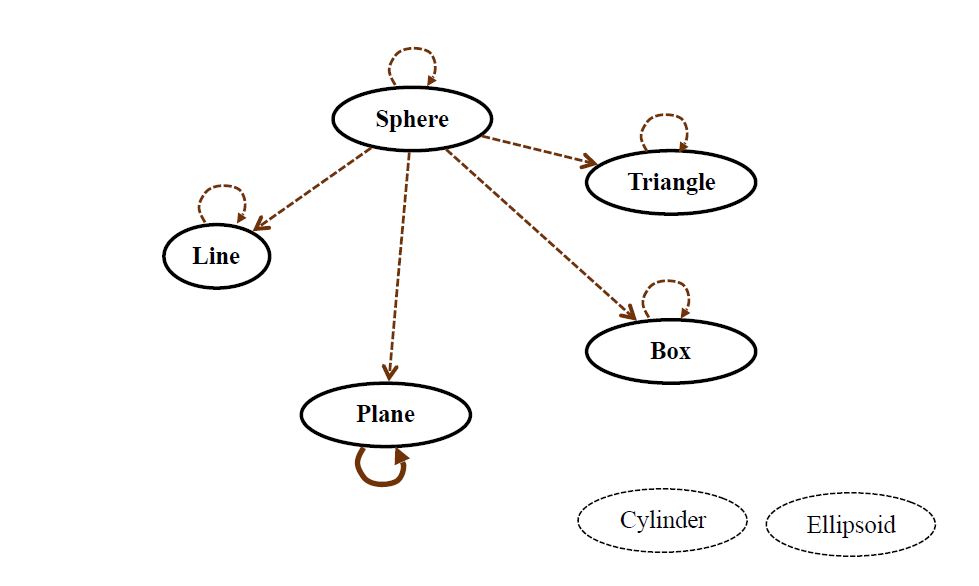
\includegraphics[width=9cm]{simpleShape.png}
					\end{figure}
			\paragraph{Multiple Objects}
				\begin{itemize}
					\item 边界体积 bounding volume
					\item 层次,空间哈希,八叉树,BSP树,OBB树  hierarchy, spatial hash, octree, BSP tree,
				\end{itemize}
				
\newpage				
\section{衣物模拟}
	\subsection{布料模拟PBD算法}在布料模拟问题中,首先要确定布料的模型。布料模型存在于一个三维世界中,设置一个端点集合V(x,y,z),当把集合V中的端点按一定的顺序互连起来时,便会形成一个连贯的面,这个面就是我们将要处理的布料,只不过目前这个布料是静态的。
		\paragraph{确定布料模型}三维空间的面经过处理模拟布料最理想。本例选用细分曲面,即按照一定顺序将顶点链接起来就是面了。
			\begin{itemize}
				\item  端点位置:Vertex(x,y,x)
				\item  链接:顺序性,约束性[拉伸,弯曲,碰撞]
				\item  真实:物理,光照,纹理
			\end{itemize}
		
		\paragraph{算法实现}如下所示为PBD核心思想:
			\begin{algorithm}[htb]
				\caption{PBD 布料模拟算法}
				\label{alg:Cloth_Simulation_PBD}
				\begin{algorithmic}[1]
					\REQUIRE ~~\\ 
					细分曲面-点集合 \\
					点的坐标
					\ENSURE ~~\\
					动态布料模拟动画
					
					\STATE 初始化数据值
							\begin{itemize}
								\item   自身限制: [各点速度$V_i$,布料起始坐标$X_i$,给点的外力$F_i$,质量$m_i$,完善否$W_i$等]
								
								\item 拉伸限制: [预测位置$tmp\_X_i$]
							\end{itemize}
					\STATE 预测点的位置
					\STATE 计算约束限制
					\STATE 更新点的坐标与速度 
					\STATE 迭代直到各个点都完成操作2-3
				\end{algorithmic}
			\end{algorithm}
\end{document} 
 		    